\documentclass[10pt]{article}

\usepackage{preprint}
\usepackage[utf8]{inputenc}
\usepackage[round,authoryear]{natbib}
\usepackage{hyperref}
\usepackage{url}
\usepackage{booktabs}
\usepackage{tabularx}
\usepackage{amsmath,amssymb,amsthm}
\usepackage{graphicx}
\usepackage{enumitem}
\usepackage{epigraph}

\hypersetup{colorlinks=true,linkcolor=refnavy,citecolor=refnavy,urlcolor=refnavy}
\graphicspath{{figures/}}
\raggedbottom
\setlength{\textfloatsep}{12pt plus 2pt minus 2pt}

\theoremstyle{plain}
\newtheorem{proposition}{Proposition}
\newtheorem{lemma}{Lemma}
\theoremstyle{remark}
\newtheorem*{remark}{Remark}
\newcommand{\R}{\mathbb{R}}
\newcommand{\U}{\mathcal{U}}
\newcommand{\M}{\mathcal{M}}
\newcommand{\D}{\mathcal{D}}
\newcommand{\Voc}{\mathcal{V}}
\newcolumntype{Y}{>{\raggedright\arraybackslash}X}
\newcolumntype{P}[1]{>{\raggedright\arraybackslash}p{#1}}
\setlist{itemsep=1pt,topsep=3pt,parsep=0pt}
\setlength{\epigraphwidth}{0.62\textwidth}
\setlength{\epigraphrule}{0pt}

\title{Defining Compositional Representations\\ by Recoverability}
\author{Karthik Singaravadivelan\\ College of Computing, Georgia Institute of Technology}
\date{October 27, 2026}
\runninghead{Defining Compositional Representations by Recoverability}
\keywords{compositionality, systematicity, representation, binding, neural networks}

\begin{document}
\maketitle

\begin{abstract}
People understand a sentence they have never heard because they can build its meaning from parts they already know, and they can take the meaning apart again into the same parts. Machine learning now calls almost any successful recombination of familiar material \emph{compositional}, and recent work has rightly separated behavioral evidence of compositionality from representational evidence. Yet what a representation must be like to count as compositional remains unsettled. Here, we formalize a simple idea: a representation is compositional when it combines parts through a relation from which every part, \emph{including a part never seen before}, can be read back in its role by the same fixed procedure. We show that the requirement of fresh parts carries the definition. On any finite vocabulary, almost every way of combining parts can be decoded by lookup, so recovery of familiar parts cannot separate composition from blending; recovery of freshly drawn parts can, and for Gaussian parts its ceiling is set exactly by the rank of the relation. Under a role-factorized relation that meets this criterion, systematicity follows from the relation instead of from the training data. We then test the definition. Analytic modes of combination match the predicted ceilings, and vector-symbolic superposition behaves like a lossy blend. Trained networks generalize to unseen pairs of familiar parts almost perfectly whether or not their states keep parts recoverable, while their transfer to new parts tracks recovery closely. Pretrained text encoders recover the nouns of familiar sentences but not of new ones. Finally, we discuss what a network must do to earn the term: allocate room for every part, learn its readout from many distinct parts, share one part code across roles, and keep its relation invertible on its own outputs.
\end{abstract}

%=====================================================================
\section{Introduction}
\label{sec:intro}

\epigraph{What we mean when we say that linguistic capacities are systematic is that the ability to produce/understand some sentences is intrinsically connected to the ability to produce/understand certain others.}{\citet{fodor1988}}

Compositionality is among the oldest ideas in the study of mind and language. \citet{frege1923} observed that we understand sentences we have never heard because we can build the sense of a sentence from parts that correspond to its words, and \citet{fodor1988} argued that the systematicity and productivity of human thought are explained by representations with constituent structure. In machine learning the idea appears as \emph{compositional generalization}, the ability to produce correct outputs for novel combinations of familiar atoms \citep{lake2018,keysers2020,kim2020cogs}. Text-to-image models are described as composing concepts into new scenes \citep{ramesh2021,okawa2023}, and language models as reasoning compositionally \citep{press2023}; yet the same models often fail to place objects in requested relations \citep{conwell2022} and express an attribute named for one object on another \citep{rassin2022}.

Most uses of the term rest on a colloquial principle that descends from Frege and \citet{montague1970}: the meaning or representation of a complex is determined by those of its parts and the way they are combined. Any system that computes a function of its inputs satisfies it, so it cannot distinguish an avocado placed \emph{on} a chair from an armchair in the shape of an avocado (Figure~\ref{fig:ops}). \citet{vegner2025} separated \emph{behavioral} compositionality, appropriate outputs for unseen combinations of familiar parts whatever the internal process, from \emph{representational} compositionality, a property of the internal states themselves, and showed that behavior does not establish the second; but they left its criterion to future work. Existing proposals measure the simplicity of a symbolic redescription \citep{elmoznino2024}, the novel structure in the best model of a whole beyond the best models of its parts \citep{elmoznino2026}, or how well an explicit composition of inferred primitives reproduces a state \citep{andreas2019}. A separate line of work proves that additive, invertible decoders generalize to unseen combinations of slots \citep{lachapelle2023,wiedemer2024}, and that linear, orthogonal factors are necessary for compositional generalization in embedding models \citep{uselis2026}. What none of these settles is when recovering parts from a representation is evidence of compositional structure, and when it is evidence only of a familiar vocabulary.

Our starting point is that a compositional representation must let its parts be read back, in their roles, by a fixed procedure that does not depend on which parts they are. This is the \emph{functional compositionality} of \citet{vangelder1990}, and the \emph{reverse compositionality} of the philosophical literature \citep{robbins2005}. Section~\ref{sec:intuition} develops this idea and shows, with one running example, why the decisive test is recovery of parts the system has never encountered.

Section~\ref{sec:definition} formalizes the definition. A relation is \emph{recoverable} when readouts from a declared class, fitted on composites of a finite vocabulary, return the parts of composites built from freshly drawn parts; it is \emph{role-factorized} when each part enters every role through one shared code. We prove that unrestricted versions of both properties are vacuous, give an exact ceiling on fresh-part recovery for linear relations, and show that under a role-factorized, recoverable relation every role reversal and every new assignment of a known part to a role follows from a single composite, the sense of necessity that \citet{fodor1990} demanded.

We test the definition in Section~\ref{sec:experiments} on analytic modes of combination, on networks trained from scratch, on recursive composition, and on six pretrained text encoders. We close in Section~\ref{sec:discussion} by stating what a network must do to count as compositional, and by discussing implications for terminology, architecture, and evaluation.

%=====================================================================
\section{Intuition for recoverable composition}
\label{sec:intuition}

\begin{figure}[t]
  \centering
  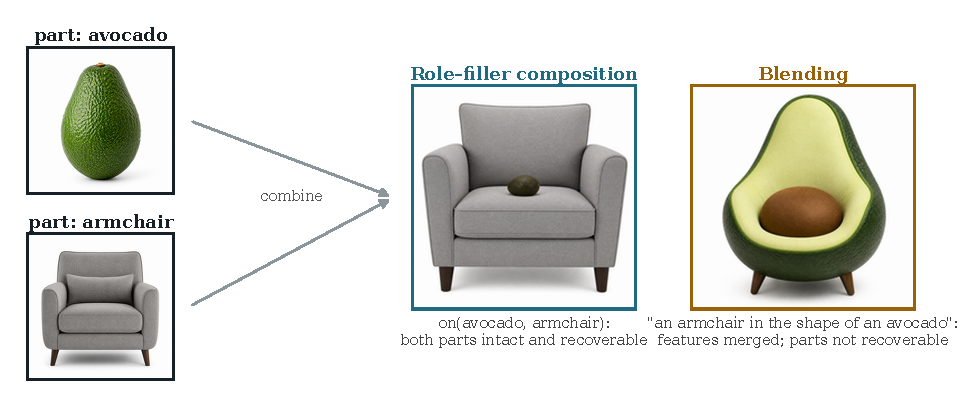
\includegraphics[width=\linewidth]{fig1_avocado.pdf}
  \caption{\textbf{Two modes of combining the same parts.} Role--filler composition places the avocado in a role of the relation \emph{on}, so that both parts remain intact and either can be read back from the whole. Blending merges the features of the two concepts into an armchair in the shape of an avocado, a prompt made familiar by DALL$\cdot$E \citep{openai2021dalle}, from which neither part can be read back. All four images were generated for this paper with Canva's text-to-image tool.}
  \label{fig:ops}
\end{figure}

Consider two ways of combining an avocado and a chair (Figure~\ref{fig:ops}). In the first, the avocado fills a role of the relation \emph{on}: the scene contains both objects intact, and an observer can say which object rests on which. In the second, the features of the two concepts merge into an avocado-shaped armchair, and neither concept survives as a part. Both are functions of the two parts, and both can be produced for a pair of parts never seen together, so the colloquial principle and behavioral tests treat them alike.

The difference lies in what can be read back. Suppose a system represents composites as vectors and combines two part vectors $x$ and $y$ by adding them. Every pair on the line $x + y = z$ yields the same composite $z$ (Figure~\ref{fig:fibers}a), so no procedure, however clever, can return the parts. A tensor product binding, $x \otimes \rho_1 + y \otimes \rho_2$ with independent role vectors, keeps one decomposition for each composite (Figure~\ref{fig:fibers}b). Three cases illustrate how this difference appears in practice.

\emph{A small vocabulary hides the difference.} If the system only ever combines parts from a vocabulary of, say, seven known vectors, few vocabulary pairs lie on any one line $x + y = z$, and a lookup over the vocabulary recovers the parts of almost every sum. The sum then looks recoverable. The recoverability comes from the sparsity of the vocabulary, not from the relation, and it disappears for a part outside the vocabulary.

\emph{Fresh parts expose it.} If we draw a new pair of parts and add them, the composite lies on a line that contains infinitely many other decompositions, and nothing distinguishes the true one. Under the tensor product, the same fixed readout that worked for familiar parts returns the new ones.

\emph{A shared procedure makes reversal necessary.} If the readout for each role is one procedure shared by all parts, and each part enters each role through one code, then reading a composite once tells the system how to build its role reversal and how to place a part it has seen only in one role into the other. Nothing about the training data is needed beyond what fixed the procedure.

For an arbitrary system, then, the question is whether some fixed readout, of a kind declared in advance, recovers each part in its role from composites of parts the readout and the system have never seen. The next section makes this precise.

%=====================================================================
\section{Defining representational compositionality}
\label{sec:definition}

\subsection{Preliminaries}

A \emph{part} is drawn from a distribution $\D$ over a space of possible parts, which may be continuous (glyphs, vectors, images) or very large (the nouns of a language). A system assigns each part $x$ a \emph{part code} $e(x) \in \R^d$, its representation of the part on its own, and assigns a composite $r(x_1, \ldots, x_k)$ of $k$ parts in roles $1, \ldots, k$ of a relation $r$ an internal state $h = g_r(x_1, \ldots, x_k) \in \R^m$. Training exposes the system to a finite \emph{vocabulary} $\Voc$ of parts drawn from $\D$; a \emph{fresh} part is a further draw from $\D$ outside $\Voc$. Composites can serve as parts, so the setup is closed under combination. A \emph{readout class} $\U$, such as affine maps, is the family of procedures we allow for recovering a part's code from a composite state; a readout $u_i \in \U$ is fitted for each role $i$ and then held fixed.

Two observations, proved in Appendix~\ref{app:proofs}, show why the class of readouts and the use of fresh parts cannot be left open. First, if the coordinates in which a relation is required to be additive are unrestricted, every invertible relation is additive in some coordinates, so additivity adds nothing to invertibility (Lemma~\ref{lem:psi}). Second, on a finite vocabulary every relation that is injective on the vocabulary is inverted exactly by a lookup table, so recovery of familiar parts cannot separate composition from blending (Lemma~\ref{lem:lookup}). Both properties have content only when the readouts and coordinates are restricted in advance and recovery is measured on parts that played no role in fitting them.

\subsection{The definition}

\begin{defbox}{Recoverable and role-factorized relations}{recoverable}
Fix a part distribution $\D$, a part code $e$, and a readout class $\U$. A relation $r$, realized in a system by $g_r$, is \emph{$\varepsilon$-recoverable} if for every role $i$ some $u_i \in \U$, fitted on composites of parts in a finite vocabulary $\Voc \sim \D$, satisfies on composites of fresh parts $x_1, \ldots, x_k \sim \D$
\begin{equation}
  \frac{\mathbb{E}\,\lVert u_i(g_r(x_1,\ldots,x_k)) - e(x_i) \rVert^2}{\mathbb{E}\,\lVert e(x) - \mathbb{E}\,e(x) \rVert^2} \;\le\; \varepsilon .
  \label{eq:recover}
\end{equation}
The relation is \emph{$\delta$-role-factorized} if there exist $c \in \R^m$ and matrices $B_1, \ldots, B_k \in \R^{m \times d}$, one per role and shared by all parts, such that the state is affine in the part codes up to a residual,
\begin{equation}
  g_r(x_1, \ldots, x_k) = c + \textstyle\sum_{i} B_i\, e(x_i) + \eta(x_1, \ldots, x_k), \qquad \mathbb{E}\,\lVert \eta \rVert^2 \le \delta\, \mathbb{E}\,\lVert g_r - \mathbb{E}\,g_r \rVert^2,
  \label{eq:factor}
\end{equation}
with the expectation again taken over fresh parts.
\end{defbox}

This criterion asks two things of a relation. Recoverability, Eq.~\eqref{eq:recover}, asks that a fixed procedure return each part in its role, and that it do so for parts outside the vocabulary from which the procedure was learned; $1 - \varepsilon$ is the fresh-part $R^2$ of the readout. Role-factorization, Eq.~\eqref{eq:factor}, asks that each part contribute the same code to every whole, transformed only by its role, which is the classical requirement that a constituent contribute the same thing to every complex in which it occurs \citep{fodor1988}, with the coordinates restricted to affine maps so that the requirement has content. Intuitively, a relation fails the first criterion when it discards information about its parts, as every blend into a space smaller than its parts must, and fails the second when what a part contributes depends on its co-parts, as in prototype combination \citep{smith1988,hampton1987}.

\begin{defbox}{Representational compositionality}{repcomp}
A system is \emph{representationally compositional} with respect to a relation $r$, relative to a declared readout class $\U$ and a declared class $\M$ of methods for finding part codes, if for some part code found under $\M$ its realization of $r$ is $\varepsilon$-recoverable and $\delta$-role-factorized, with $\varepsilon$ and $\delta$ no worse than those of a reference role--filler operator applied to the same part codes. The relation is \emph{productive to depth $n$} if the same holds when the parts are themselves composites of depth up to $n - 1$, with the same readouts applied recursively.
\end{defbox}

Note that Definition~\ref{def:repcomp} is graded and relative. It is graded because $\varepsilon$ and $\delta$ are continuous, and we calibrate them against reference operators built from the system's own part codes, since the best attainable values depend on the parts and on the readout class (Section~\ref{sec:pretrained}). It is relative to $\U$ and $\M$ because the decomposition must be found by search; a negative result is therefore reported as the absence of a decomposition under declared methods, and the methods must be validated on systems whose decomposition is known. Restricting $\U$ is not a convenience: with unrestricted readouts, as with unrestricted causal alignment maps \citep{sutter2025}, any injective system passes.

\begin{notebox}{What the definition does not require}{scope}
The definition does not require that parts be interpretable to people, that constituents be tokened as separate symbols \citep{fodor1990}, or that the part code be the input embedding; part codes found without supervision are admitted under $\M$. Nor does it require recovery at unbounded depth: a state of fixed dimension cannot invertibly encode trees of unbounded depth over continuous parts (Proposition~\ref{prop:depth}), so productivity is reported as a curve over depth, and its limits, as \citet{fodor1988} argued, are matters of performance.
\end{notebox}

\begin{figure}[t]
  \centering
  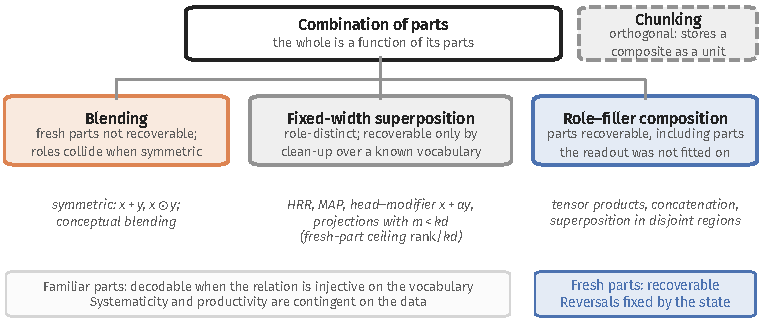
\includegraphics[width=\linewidth]{fig_taxonomy.pdf}
  \caption{\textbf{Modes of combination, sorted by what survives fresh parts.} Every mode satisfies the colloquial principle. Blends discard their parts or confuse their roles. Fixed-width superposition, which includes holographic reduced representations (HRR) and other vector-symbolic architectures, keeps roles distinct but returns parts only by clean-up over a known vocabulary; its fresh-part recovery is bounded by the rank of the relation (Proposition~\ref{prop:ceiling}). Only role--filler composition, which includes superposition in disjoint regions, recovers parts never seen before and so satisfies Definition~\ref{def:repcomp}. Chunking stores a composite of any mode as a unit and is orthogonal to the distinction.}
  \label{fig:taxonomy}
\end{figure}

\subsection{What the definition accounts for}
\label{sec:consequences}

Appendix~\ref{app:proofs} proves eight results; we state the four that carry the argument.

\textbf{Blends cannot be read back, and how much they lose is computable.} If a relation is linear, $g(x_1, \ldots, x_k) = A x$ with $A = [A_1 \cdots A_k]$, and its image is smaller than the space of its parts, each composite has an affine family of decompositions of dimension $kd - \mathrm{rank}\,A$ (Proposition~\ref{prop:fiber}). For Gaussian parts the loss is exact: no readout of any kind recovers role $i$ with $R^2$ above $\mathrm{tr}(A_i^{\top}(AA^{\top})^{+}A_i)/d$, and the average over roles is $\mathrm{rank}\,A/(kd)$ (Proposition~\ref{prop:ceiling}). The ceiling is $0.8$ for role~1 of $x + 0.5y$, $0.5$ for either role of $x + y$, and $m/(kd)$ for a generic projection into $m < kd$ dimensions. Intuitively, a blend keeps only as many dimensions of its parts as its image has room for.

\textbf{Familiar parts can be decoded anyway.} When parts come from a finite vocabulary, a non-invertible relation can be injective on that vocabulary, and its parts can be decoded by clean-up \citep{plate1995,plate2003,frady2018}. This recoverability comes from the sparsity of the vocabulary rather than from the relation, and it fails for parts outside the vocabulary. The same holds for readouts learned from a vocabulary: a linear readout fitted on composites whose part codes do not span $\R^d$ is undetermined on the remaining directions (Proposition~\ref{prop:span}), so a readout, or a network's own decoding procedure, must be learned from enough distinct parts before it can recover new ones.

\textbf{Under role-factorization, systematicity is necessary.} If a relation is role-factorized and recoverable with $\delta = \varepsilon = 0$ and the stacked matrix $[B_1 \cdots B_k]$ has full column rank, then every role reversal and every assignment of a known part to a role it has never occupied is an affine function of a single composite containing it (Proposition~\ref{prop:systematic}). Intuitively, reading a composite once yields each part's code, and the shared role maps say where each code goes in any other arrangement. This is the necessity that \citet{fodor1990} required of a compositional architecture, obtained from the relation and not from the tokening of constituents. Without role-factorization, observed composites constrain unobserved ones only when the set of observed pairs connects every part to every role (Proposition~\ref{prop:separable}), so systematic behavior on a new role assignment depends on the training data and is in this sense contingent \citep{aizawa2003}.

\textbf{Productivity requires invertibility on the relation's own outputs.} A nested linear blend of depth $n$ loses at least $(2^n - 1)d$ dimensions of its leaves (Proposition~\ref{prop:depth}). A relation that is invertible on composites of parts need not be invertible on composites of composites, which are drawn from a different distribution; productivity therefore requires that the relation remain recoverable when applied to its own outputs, a property we test directly.

\subsection{Relationship to other accounts}
\label{sec:related}

\textbf{Identifiability of additive decoders.} Our two conditions are not new as mathematics. Additive decoders, which render each slot separately and sum the results, together with an encoder that inverts the decoder on recombined slots, are the sufficient conditions under which object-centric models provably generalize to unseen combinations of slots \citep{brady2023,lachapelle2023,wiedemer2024}, and \citet{wiedemer2023} locate compositional generalization in the data-generating process rather than the data. Our separability is their additivity with affine coordinates, our recoverability is their consistency, and their caveat that additivity fails under occlusion is our prediction for overlapping roles (Section~\ref{sec:networks}). Two things are new. We use the conditions to \emph{define} a representational property and not as sufficient conditions for a behavioral one, and we require recovery of fresh parts, which separates what the relation guarantees from what a vocabulary supplies.

\textbf{Necessary structure.} \citet{uselis2026} argue that compositional generalization in embedding models requires representations that decompose linearly into per-concept components, orthogonal across concepts. Their result runs from behavior to structure; Proposition~\ref{prop:systematic} runs from structure to behavior. Together they suggest that role-factorized recoverability is close to both necessary and sufficient for systematic generalization over parts, and our experiments find the two tightly coupled in trained networks. \citet{schug2024} show that a number of training tasks linear in the number of modules suffices when the training support is connected, which is the learning-theoretic analogue of Proposition~\ref{prop:separable}, and \citet{lippl2025} show that kernel models generalize compositionally only through conjunction-wise additive computations, with a ``memorization leak'' that corresponds to our residual $\eta$.

\textbf{Decodability and generalization.} Measuring whether a readout trained on some conditions transfers to held-out conditions is standard in neuroscience as cross-condition generalization \citep{bernardi2020,ito2022}, and linear decodability of constituents accompanies compositional generalization as models scale \citep{redhardt2025}. Decodable, disentangled factors do not by themselves ensure that a decoder generalizes \citep{montero2021}, and models can generalize without compositional messages \citep{chaabouni2020}; these are the two off-diagonal cells of Table~\ref{tab:twobytwo}. Discovered tensor-product decompositions of trained networks \citep{mccoy2019,soulos2020}, binding identifiers in language models \citep{feng2024}, and interchange interventions \citep{geiger2021,geiger2024das} are methods that $\M$ can contain. What we add is the requirement that the readouts be evaluated on parts outside the vocabulary from which they and the system were fitted.

\textbf{Compression-based accounts.} \citet{elmoznino2024} define representational compositionality by the description length of a representation under a simple symbolic redescription, and \citet{elmoznino2026} measure the novel structure in the best model of a whole that the best models of its parts cannot recover. Both are compression-based and neither requires that parts be read back from the whole; a fixed-width superposition over a small vocabulary compresses well and is decodable by clean-up, and it fails our criterion only on fresh parts. The accounts are complementary: theirs asks how much shared structure a decomposition reveals, ours asks whether the decomposition can be recovered by a fixed procedure.

\textbf{The classical debate.} \citet{fodor1990} objected that constituents which are not tokened cannot cause systematic processing. Proposition~\ref{prop:systematic} answers that the necessity they wanted comes from the relation: when one role-factorized, recoverable relation serves every filler and role, the ability to build and read any arrangement follows from the ability to read one. \citet{goodale2026} restate the challenge as one about what an architecture guarantees by default, and \citet{woydt2025} argue that meta-learning \citep{lake2023} has not yet produced human-like systematicity. Our criterion is a property of states, not of architectures, so a network can meet it by training; Section~\ref{sec:discussion} returns to this point.

\begin{table}[t]
  \caption{Behavioral and representational compositionality vary independently \citep[cf.][]{vegner2025}.}
  \label{tab:twobytwo}
  \centering\small
  \begin{tabularx}{\linewidth}{@{}P{3.2cm}YY@{}}
    \toprule
    & Behavior succeeds on new combinations and new parts & Behavior fails \\
    \midrule
    Parts recoverable from fresh composites & Compositional; systematicity follows from the relation & Failure of performance, such as a poor decoder \citep{montero2021} \\
    Parts recoverable only from familiar composites & Imitation; systematicity is contingent on the data \citep{chaabouni2020} & Blending that fails \\
    \bottomrule
  \end{tabularx}
\end{table}

%=====================================================================
\section{Testing recoverability}
\label{sec:experiments}

The definition is useful only if it separates systems that differ in the way it claims. We ask four questions: \emph{do analytic modes of combination meet the predicted ceilings? do networks trained from scratch recover fresh parts, and does that predict how they behave? does recovery survive recursion? and do pretrained encoders recover the parts of new sentences?} Each experiment below is fully characterized by:
\begin{itemize}
  \item \textbf{Composites:} the parts, their distribution $\D$, and the relation;
  \item \textbf{Readouts:} the declared class $\U$, fitted on composites of a vocabulary $\Voc$ and evaluated on held-out pairs of vocabulary parts, on parts in roles they never occupied, and on fresh parts;
  \item \textbf{Measures:} recovery ($R^2$ of the part code or identification among candidates) and, for systems that act, behavior on the same splits.
\end{itemize}
Methods are summarized below; Appendix~\ref{app:protocol} gives full details, and every number is a mean over seeds with standard errors in the figures.

\subsection{Calibration on analytic modes of combination}
\label{sec:calibration}

\textbf{Composites.} Parts are Gaussian vectors in $\R^{16}$. We combine pairs with fourteen operators (Figure~\ref{fig:calibration}a): concatenation and a tensor product with two random roles (role--filler); random linear projections into $m = 0.5$ to $1.5$ times $kd = 32$ dimensions, HRR and MAP binding in 16 dimensions, and weighted addition $x + 0.5y$ (fixed-width superposition); $x + y$ and $x \odot y$ (symmetric blends); and a random $\tanh$ layer of three widths.

\textbf{Readouts.} We fit ridge (linear) and two-layer MLP readouts for the role-1 part on 6{,}000 composites of a vocabulary of $V$ parts, and evaluate them on unseen pairs of vocabulary parts and on pairs of fresh parts. A lookup decoder matches each composite to the table of all composites of a candidate set, given the candidates.

\textbf{Results.} We ran 5 seeds for each $V \in \{4, \ldots, 128\}$. Given the candidates, lookup identifies the role-1 part of every operator that is injective on the vocabulary, including half-rank projections, HRR, and the narrowest $\tanh$ layer, with accuracy 1.00; only the symmetric blends fall to 0.50, a role collision (Figure~\ref{fig:calibration}a). Recovery of familiar parts therefore does not discriminate. Recovery of fresh parts does, and it matches the ceiling of Proposition~\ref{prop:ceiling} (Figure~\ref{fig:calibration}b): $R^2 = 1.00$ for concatenation, the tensor product, and full-rank projections; $0.69$ and $0.45$ for projections at $m/kd = 0.75$ and $0.5$; $0.80$ for $x + 0.5y$, whose ceiling is $0.80$; $0.50$ for $x + y$; and $0.42$ and $0.45$ for HRR and MAP, which behave exactly like a half-rank projection. Vector-symbolic superposition is therefore not invertible in the sense of Definition~\ref{def:recoverable}; it is decodable over a vocabulary.

Figure~\ref{fig:calibration}c shows that the readout must itself be learned from enough parts: with $V = 8$ parts in $\R^{16}$, the linear readout of concatenated parts, which is perfect in principle, recovers fresh parts with $R^2 = 0.05$ while recovering familiar ones perfectly; it reaches $0.90$ at $V = d = 16$ and $1.00$ at $V = 32$ (Proposition~\ref{prop:span}). Figure~\ref{fig:calibration}d shows that the readout class matters: MLP readouts fit familiar parts at least as well as linear ones but transfer worse to fresh parts, for instance $0.10$ against $0.45$ at $m/kd = 0.5$. A flexible readout memorizes the vocabulary, which is why $\U$ must be declared and restricted. These recovery profiles serve as the references against which the states of trained systems are placed.

\begin{figure}[t]
  \centering
  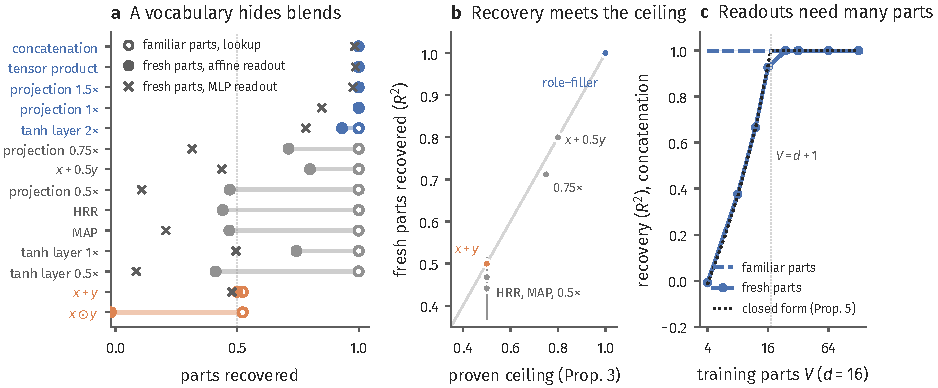
\includegraphics[width=\linewidth]{fig_calibration.pdf}
  \caption{\textbf{Calibration on analytic modes of combination.} \textbf{a.} Given a set of candidate parts, a lookup over their composites identifies the role-1 part of every operator that is injective on the vocabulary (blue: role--filler; grey: fixed-width superposition), and fails only for symmetric blends (orange), whose roles collide; $V = 32$. \textbf{b.} A linear readout fitted on vocabulary composites and evaluated on fresh parts recovers exactly what the ceiling of Proposition~\ref{prop:ceiling} allows; HRR and MAP fall with half-rank projections. $V = 128$. \textbf{c.} Recovery of familiar (dashed) and fresh (solid) parts as a function of the number of training parts; the readout transfers only once the parts span the part space ($V \ge d = 16$). \textbf{d.} MLP readouts transfer worse than linear ones to fresh parts. \textbf{Seeds.} Means over 5 seeds; bands and error bars show standard errors.}
  \label{fig:calibration}
\end{figure}

\subsection{Networks trained from scratch}
\label{sec:networks}

\textbf{Composites.} A part is a latent $z \in \R^{8}$ rendered as an $8 \times 8$ glyph by a fixed random nonlinear generator, and a composite of two parts is rendered on an $8 \times 16$ canvas under one of three relations (Figure~\ref{fig:networks}a): \textsc{beside} places the glyphs in disjoint regions; \textsc{over} draws both in the same region, the second mirrored; and \textsc{occlude} draws the second glyph at half scale over the brightest quadrant of the first, so that where a part goes depends on its host. \textsc{beside} and \textsc{over} are exactly additive in the rendered pixels; \textsc{occlude} is not (interaction 11--14\% of composite variance). All three are invertible in principle.

\textbf{Task and systems.} An encoder sees only a composite and writes a bottleneck state $h \in \R^m$; a decoder receives $h$ and a flag for a target relation and must render the same parts, in the same roles, under that relation. The state $h$ is therefore the system's representation of the composite. We compare an MLP, a CNN, and a transformer over pixel columns, each with an MLP decoder, and a \emph{role--filler decoder} that splits $h$ into two slots, decodes each with one shared glyph decoder, and renders the relation with a fixed renderer. A quarter of the vocabulary never occupies role~2 in training (Hadley's strong systematicity), and a random fifth of the remaining pairs is withheld as a difficulty-matched baseline. We vary $m \in \{8, 16, 32, 64\}$ around $kq = 16$, the dimension of a pair of latents, and $V \in \{8, 16, 32, 64\}$, with 10 seeds each.

\textbf{Readouts.} A ridge readout is fitted from $h$ to each role's glyph on training composites and evaluated on held-out pairs, new-role pairs, and pairs of fresh glyphs.

\textbf{Results.} Every architecture reproduces unseen pairs of familiar glyphs well, with output $R^2$ between 0.86 and 1.00 in every condition except the transformer trained on eight glyphs (0.55--0.65; Figure~\ref{fig:networks}b,c, dashed). Behavior on held-out pairs therefore barely separates the systems. Transfer to fresh glyphs does: it is limited by the width of the state, with $R^2$ between 0.58 and 0.68 at $m = 8 < kq$ against 0.83 to 0.90 at $m \ge 16$ (Figure~\ref{fig:networks}b), and above all by the number of distinct training parts, rising from at most 0.30 at $V = 8$ (negative for the transformer) to 0.84--0.90 at $V = 64$, with the state as wide as $m = 64$ (Figure~\ref{fig:networks}c). The MLP, CNN, and role--filler networks trained on eight parts thus fall in the imitation cell of Table~\ref{tab:twobytwo}: they generalize to unseen pairs ($R^2$ 0.86--0.99) while their states do not let new parts be read back. The width effect is the ceiling of Proposition~\ref{prop:ceiling} acting in a trained network; the vocabulary effect is Proposition~\ref{prop:span} acting on the network's own decoding procedure.

Across all runs, the fresh-part recovery of the state predicts transfer to fresh parts with correlation $r = 0.94$, while it predicts behavior on held-out pairs only weakly ($r = 0.61$; Figure~\ref{fig:networks}d). The role--filler decoder, which shares one glyph decoder across roles, is the best on parts in new roles at the smallest vocabulary (output $R^2$ 0.32--0.33 at $V = 8$, against 0.11--0.27 for the MLP and CNN and below zero for the transformer), as role-factorization predicts; by $V = 16$ the CNN matches it (0.73--0.74 against 0.72--0.81). It transfers no better to fresh parts, because its encoder is unconstrained. Interaction between parts lowers transfer for every architecture: at $m = V = 64$, fresh-part $R^2$ falls from 0.84--0.91 under \textsc{beside} to 0.61--0.80 under \textsc{occlude} (Figure~\ref{fig:networks}e), and the states carry 1--4\% interaction against 11--14\% in the input, so the networks approximate the non-additive relation by an additive one. Finally, behavior on new roles varies widely across seeds when the vocabulary is small and hardly at all when it is large (Figure~\ref{fig:networks}f), the signature of systematicity that is contingent on training \citep{mccoy2020berts}.

\begin{figure}[t]
  \centering
  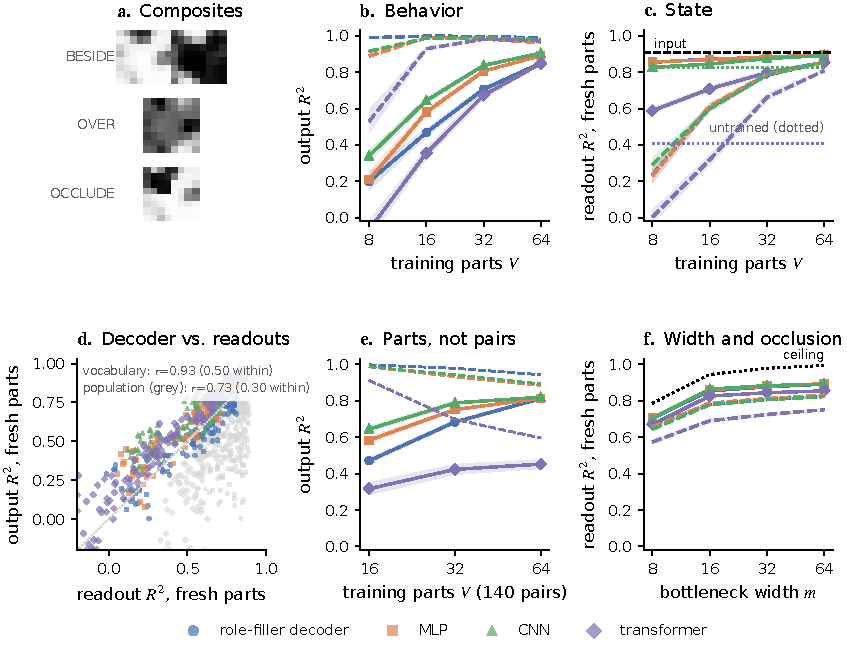
\includegraphics[width=\linewidth]{fig_networks.pdf}
  \caption{\textbf{Networks trained from scratch on glyph composites.} \textbf{a.} One pair of glyphs under the three relations. \textbf{b.} Output $R^2$ on unseen pairs of familiar glyphs (dashed) and on pairs of fresh glyphs (solid) as a function of the width of the state, for four architectures ($V = 64$); fresh-part transfer drops below the width of a pair of latents, $m = kq$. \textbf{c.} The same as a function of the number of training glyphs ($m = 64$): unseen pairs are solved from eight glyphs, new glyphs are not. \textbf{d.} Each point is one run. Recovery of fresh glyphs from the state (ridge readout) predicts output $R^2$ on fresh glyphs (colored), but not on held-out pairs (grey), which is near ceiling throughout. \textbf{e.} Fresh-glyph transfer by input relation ($m = V = 64$); the non-additive \textsc{occlude} costs every architecture. \textbf{f.} Standard deviation across seeds of output $R^2$ for glyphs in a role they never occupied ($m \ge 32$). \textbf{Seeds.} 10 seeds per condition (5 for \textsc{occlude}); bands and error bars show standard errors.}
  \label{fig:networks}
\end{figure}

\subsection{Recursion}
\label{sec:depth}

\textbf{Composites.} Balanced binary trees of depth $n$ have leaves drawn from a vocabulary of $V$ Gaussian parts in $\R^8$, or fresh.

\textbf{Systems and readouts.} A recursive auto-associative memory \citep{pollack1990} applies one learned composer $\R^w \times \R^w \to \R^w$ at every node and one learned decomposer recursively, trained end to end on trees of depth 1 and 2. We compare HRR with unitary roles of the same width, whose leaves are decoded by recursive unbinding and identified by clean-up.

\textbf{Results.} We ran 5 seeds for each width $w$ and $V \in \{16, 64\}$. Within the trained depths the learned composer recovers fresh leaves almost perfectly whenever its width allows ($R^2 \ge 0.95$ for $w \ge 2^n d$), so it meets Definition~\ref{def:recoverable} at depth 1 and 2. At depth 3 it fails even with ample width: at $w = 256$, where the ceiling of Proposition~\ref{prop:depth} is still 1, fresh-leaf $R^2$ is 0.26 and familiar leaves are identified only 49\% of the time with $V = 16$ (0.41 and 27\% with $V = 64$; Figure~\ref{fig:depth}a,b). The composer learned a relation that is invertible on the composites it was trained on, not on its own outputs. HRR degrades smoothly instead, from perfect identification at depth 1 to 49\% at depth 3 and 20\% at depth 5 at the same width, as noise from superposed bindings accumulates. Neither system is productive in the sense of Definition~\ref{def:repcomp}; they fail in different ways, and the depth curve shows which.

\subsection{Pretrained text encoders}
\label{sec:pretrained}

\textbf{Composites.} Sentences place two nouns in the roles of a relation: ``a $x$ on a $y$'', ``a $x$ to the left of a $y$'', and the symmetric control ``a $x$ and a $y$''. We use 305 concrete nouns, 170 for fitting readouts and 80 as fresh parts. The part code of a noun is the model's state for ``a $x$'', reduced to 32 principal components fitted on the training nouns.

\textbf{Systems and readouts.} We examine the text encoders of CLIP ViT-B/32 \citep{radford2021clip} and of Stable Diffusion 1.5 (CLIP ViT-L/14; \citealp{rombach2022}), T5-small and T5-base \citep{raffel2020t5}, BERT-base \citep{devlin2019bert}, and GPT-2 \citep{radford2019gpt2}, at a middle layer, the final layer, and the pooled output, and report each model's best layer. Ridge readouts map the composite state to each role's part code. To calibrate, we apply the identical pipeline to two reference operators built from each model's own part codes: concatenation, which is role--filler, and the sum, a symmetric blend.

\textbf{Results.} We ran 3 seeds per model. The pipeline recovers fresh nouns from the concatenation reference with $R^2$ between 0.97 and 1.00 for every model, so the method can detect recoverability with these part codes. Every model looks compositional on the training nouns, with $R^2$ between 0.82 and 1.00 (Figure~\ref{fig:depth}c). On fresh nouns the picture changes: the two CLIP encoders fall far below even the symmetric-sum reference ($R^2 = -1.21$ and $-0.92$, against $0.47$), BERT and T5-small reach 0.12 and 0.20, and only GPT-2 and T5-base exceed the sum reference, at 0.79 and 0.57, both at a middle layer. Every model assigns roles to fresh nouns better than the sum reference, and CLIP's composite states are nearly invariant to role reversal (normalized reversal similarity 0.91), consistent with reports that CLIP behaves like a bag of words \citep{yuksekgonul2023}. Under the declared readouts and part codes, then, no encoder we tested meets the criterion; the relations of the CLIP encoders that condition text-to-image models are the furthest from it.

\begin{figure}[t]
  \centering
  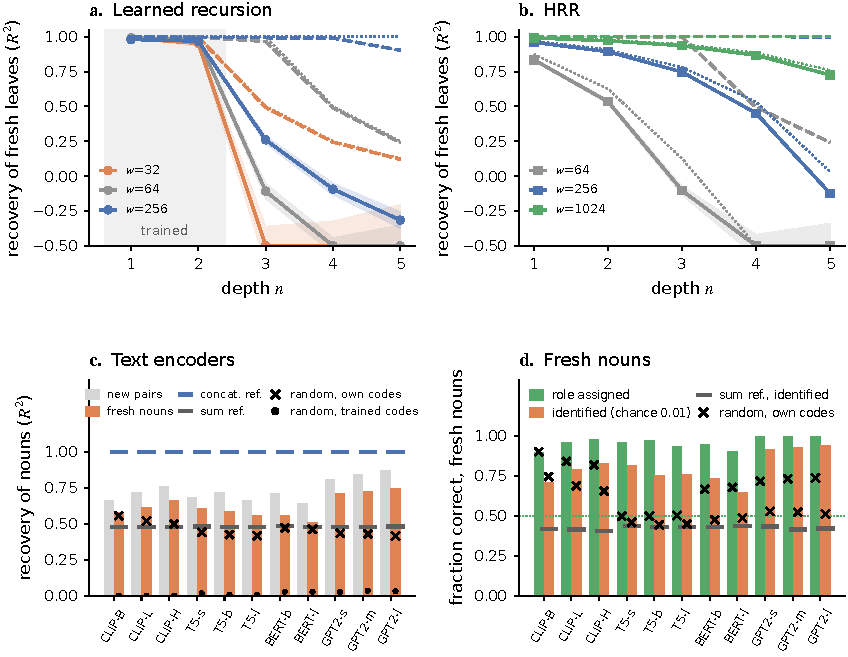
\includegraphics[width=\linewidth]{fig_depth_pretrained.pdf}
  \caption{\textbf{Recursion and pretrained text encoders.} \textbf{a.} Recovery of fresh leaves by a learned recursive composer of width $w$, trained on depths 1 and 2 (shaded); dotted lines show the ceiling of Proposition~\ref{prop:depth}. The composer fails at depth 3 even when the ceiling is 1. \textbf{b.} Identification of familiar leaves for the learned composer and for HRR with clean-up. \textbf{c.} Recovery of nouns from sentence states at each model's best layer: training nouns (grey) and fresh nouns (orange), against references built from the same model's part codes (blue: concatenation; dark grey: sum). Values below $-1$ are clipped. \textbf{d.} On fresh nouns, the fraction of readouts that assign the right role and the identification of the noun among 80 candidates. \textbf{Seeds.} 5 seeds (a, b) and 3 seeds (c, d) per condition; bands show standard errors.}
  \label{fig:depth}
\end{figure}

%=====================================================================
\section{Discussion}
\label{sec:discussion}

We proposed that a representation is compositional when it combines parts through a relation from which every part, including a part never seen before, can be read back in its role by a fixed procedure of a declared kind, and when each part enters every role through one shared code. Formally, the relation is recoverable and role-factorized over fresh parts, relative to declared readouts and declared methods for finding parts. The requirement of fresh parts is what gives the definition content: on a finite vocabulary nearly every mode of combination can be decoded, and the evidence usually offered for compositional representations, recovery of familiar parts and generalization to unseen pairs of them, is satisfied by systems whose states lose their parts.

\textbf{What a network must do.} Our results suggest four requirements, each tied to a proposition and an experiment. \emph{First, the composite state must have room for every part:} a state narrower than the parts it combines is a blend, and its fresh-part recovery is capped by its rank (Proposition~\ref{prop:ceiling}; Figures~\ref{fig:calibration}b and \ref{fig:networks}b). \emph{Second, the procedure for reading parts must be learned from many distinct parts, not many combinations:} a network trained on eight glyphs solves every unseen pair and fails on new glyphs, because its decoding procedure is undetermined outside the span of the parts it saw (Proposition~\ref{prop:span}; Figure~\ref{fig:networks}c). Coverage of combinations, which benchmarks reward, is not the variable that matters. \emph{Third, parts should enter every role through one code:} sharing the part decoder across roles made new role assignments most reliable at the smallest vocabulary, and it is the condition under which systematicity follows from the relation (Proposition~\ref{prop:systematic}). \emph{Fourth, the relation must stay invertible on its own outputs:} a composer that is invertible at the depths it was trained on can still fail one level deeper (Figure~\ref{fig:depth}a). A network that meets all four, verified on fresh parts against references built from its own part codes, has earned the term in our sense; one that meets only the behavioral tests should be described as generalizing compositionally.

\textbf{Terminology.} Behavioral evidence should be reported as compositional generalization, with the split it was measured on; the bare term should be reserved for systems whose parts are recoverable from composites of fresh parts. Reports of recovered parts should state the readout class and whether the parts were in the vocabulary used to fit the readout.

\textbf{Necessity and architecture.} \citet{fodor1990} asked that systematicity follow from the architecture. Our criterion is a property of states, and a trained network can come to satisfy it; within such a network, systematic behavior is guaranteed by the relation it learned, but whether it learns that relation remains contingent on training, as the seed spread at small vocabularies shows. Architectures that build in role-factorized slots move part of the guarantee into the architecture, but our role--filler decoder shows that the encoder must still learn a recoverable relation. Whether any training regime reliably leads a network without built-in roles to a role-factorized, recoverable relation under overlapping roles is open.

\textbf{People.} Human evidence points to recoverable composition, used selectively. People encode agent and patient in separate codes that generalize across verbs \citep{frankland2015}, represent novel objects as compositions of known elements \citep{schwartenbeck2023}, use a newly learned word in combinations they have never seen \citep{lake2019}, and endorse inferences across arbitrary contents \citep{rips1994}; yet belief overrides validity \citep{evans1983} and concepts are often blended \citep{wisniewski1997}. Appendix~\ref{app:human} collects this evidence into a reference profile against which systems can be compared.

\textbf{Future work and limitations.} Our trained networks are small and our domains synthetic, chosen so that every state could be examined and fresh parts could be drawn; the pretrained encoders were probed with one declared part code, the state of a noun in isolation, and a linear readout, and a richer class $\M$, including discovered tensor-product decompositions \citep{soulos2020} or contextual token states, might find a decomposition we did not. Can unsupervised methods reliably discover the part codes of a large network, so that a negative result reflects the network and not the method? Does scale, which brings decodability of constituents \citep{redhardt2025}, also bring recovery of fresh parts? And can a system keep its parts recoverable while matching networks in perception and graded similarity? Structured systems that build in parts of the criterion, such as DORA \citep{doumas2022}, CHREST \citep{gobet2000}, and \textsc{Trellis} \citep{singaravadivelan2026}, are natural next candidates for the same tests.

\bibliographystyle{apalike}
\bibliography{references}

%=====================================================================
\clearpage
\appendix
\titleformat{\section}{\large\bfseries}{Appendix \thesection}{0.8em}{}

\section{Formal results}
\label{app:proofs}

Throughout, a relation acts on parts $x_1, \ldots, x_k$ with codes in $\R^d$ and produces a state in $\R^m$; we write $x = (x_1, \ldots, x_k) \in \R^{kd}$ when the codes are stacked.

\begin{figure}[h]
  \centering
  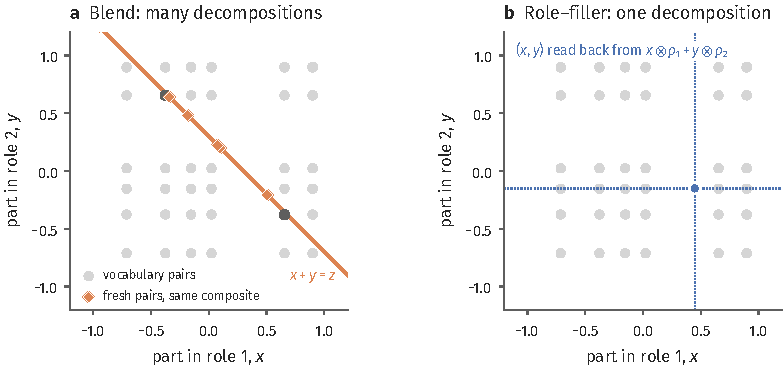
\includegraphics[width=0.9\linewidth]{fig_fibers.pdf}
  \caption{\textbf{Why a vocabulary hides a blend.} \textbf{a.} Under $x + y$, every pair on the line yields the same composite. Few pairs of a finite vocabulary (dark points) fall on any one line, so the parts of familiar composites can be decoded, but fresh pairs (diamonds) can lie anywhere on it. \textbf{b.} Under a role--filler relation each composite has one decomposition, for familiar and fresh parts alike.}
  \label{fig:fibers}
\end{figure}

\begin{lemma}[Unrestricted coordinates make separability vacuous]
\label{lem:psi}
Call $g$ separable if $\psi(g(x_1, \ldots, x_k)) = \sum_i \varphi_i(x_i)$ for some invertible $\psi$ and some maps $\varphi_i$. If $\psi$ is unrestricted, every injective $g$ is separable.
\end{lemma}

\begin{proof}
Let $\varphi_i(x_i)$ place $x_i$ in the $i$-th block of $\R^{kd}$ and zeros elsewhere, so that $\sum_i \varphi_i(x_i) = x$. On the image of $g$ define $\psi = g^{-1}$, which exists because $g$ is injective; then $\psi(g(x)) = x = \sum_i \varphi_i(x_i)$.
\end{proof}

\noindent
Intuitively, separability in arbitrary coordinates says only that the parts can be recovered, so it cannot add anything to invertibility. Definition~\ref{def:recoverable} therefore fixes the coordinates to be affine (Eq.~\ref{eq:factor}). Whether a relation is additive under some monotone transformation of each coordinate is the classical question of additive conjoint measurement \citep{luce1964}, which characterizes it by cancellation conditions; a declared class of coordinate maps between affine and unrestricted is a natural extension.

\begin{lemma}[Lookup decodes any relation that is injective on a vocabulary]
\label{lem:lookup}
Let $\Voc$ be finite and let $g$ be injective on $\Voc^k$. Then the readout that matches a state to the stored table $\{g(t) : t \in \Voc^k\}$ returns every part of every composite of vocabulary parts.
\end{lemma}

\begin{proof}
Each state in the table has exactly one preimage in $\Voc^k$.
\end{proof}

\noindent
Every relation except those with collisions on the vocabulary passes this test, including random codes that have no structure at all; Figure~\ref{fig:calibration}a confirms it for every injective operator we tried.

\begin{proposition}[Role collisions]
\label{prop:blend}
If $g(a, b) = g(b, a)$ for some parts $a \neq b$, no readout of the state can determine which of $a$ and $b$ occupies which role.
\end{proposition}

\begin{proof}
Any function of identical states returns identical values.
\end{proof}

\begin{proposition}[Non-identifiability of linear blends]
\label{prop:fiber}
Let $g(x) = Ax$ with $A = [A_1 \cdots A_k] \in \R^{m \times kd}$, which covers symmetric blending, weighted addition, superposition, and HRR or MAP binding with fixed roles. If $\mathrm{rank}\,A < kd$, which holds whenever $m < kd$, then for every composite $z$ in the image of $g$ the parts with $g(x) = z$ form an affine subspace of dimension $kd - \mathrm{rank}\,A \geq 1$, and no readout recovers the parts of every composite.
\end{proposition}

\begin{proof}
If $Ax_0 = z$, the solutions of $Ax = z$ are $x_0 + \ker A$, of dimension $kd - \mathrm{rank}\,A$ by rank--nullity. Any nonzero $n \in \ker A$ has a nonzero block $n_i$, so $x_0$ and $x_0 + n$ share the composite but differ in their $i$-th part.
\end{proof}

\begin{remark}
No continuous map from $\R^{kd}$ to $\R^m$ with $m < kd$ is injective, so the conclusion extends to continuous nonlinear relations; discontinuous injections exist but are not stable under any noise. A tensor product with linearly independent roles has $\mathrm{rank}\,A = kd$.
\end{remark}

\begin{proposition}[Ceiling on fresh-part recovery]
\label{prop:ceiling}
Let $x \sim \mathcal{N}(0, I_{kd})$ and $z = Ax$. The readout that minimizes the expected squared error of $x_i$ given $z$, among all measurable functions, is linear, and its $R^2$ for role $i$ is
\begin{equation}
  R^2_i = \frac{1}{d}\,\mathrm{tr}\big(A_i^{\top} (A A^{\top})^{+} A_i\big), \qquad \frac{1}{k}\sum_i R^2_i = \frac{\mathrm{rank}\,A}{kd}.
\end{equation}
\end{proposition}

\begin{proof}
$x$ and $z$ are jointly Gaussian with $\mathrm{Cov}(x, z) = A^{\top}$ and $\mathrm{Cov}(z) = AA^{\top}$, so $\mathbb{E}[x \mid z] = A^{\top}(AA^{\top})^{+}z$, which is linear and is the minimum-mean-square-error estimator over all functions. Its residual covariance is $I - P$ with $P = A^{\top}(AA^{\top})^{+}A$, the orthogonal projection onto the row space of $A$. The variance of $x_i$ explained is the trace of the $i$-th diagonal block of $P$, which is $\mathrm{tr}(A_i^{\top}(AA^{\top})^{+}A_i)$, out of a total of $d$. Summing over blocks gives $\mathrm{tr}\,P = \mathrm{rank}\,A$.
\end{proof}

\noindent
Intuitively, a blend keeps only the components of its parts that lie in the row space of the relation. For $x + \alpha y$ the ceiling is $1/(1 + \alpha^2)$ for role~1 and $\alpha^2/(1 + \alpha^2)$ for role~2; for $x + y$ it is $1/2$ for each; for HRR or MAP binding of two parts in $d$ dimensions with fixed roles it averages $1/2$; and for a generic projection into $m < kd$ dimensions it is close to $m/(kd)$ for each role. Figure~\ref{fig:calibration}b compares these values with fitted readouts.

\begin{proposition}[Readouts are determined only on the span of the training parts]
\label{prop:span}
Let a readout $u(h) = Wh + b$ be fitted by least squares on states of a role-factorized relation with $\delta = 0$ and full-rank $[B_1 \cdots B_k]$, using composites whose role-$i$ part codes span a subspace $S \subset \R^d$ after centering. Then every affine readout that fits the training composites exactly agrees with the true inverse on composites whose role-$i$ code lies in $S$, and the fitted readouts can differ arbitrarily on codes with a component orthogonal to $S$. In particular, recovery of fresh parts is guaranteed only if $\dim S = d$, which requires at least $d + 1$ distinct parts in role $i$.
\end{proposition}

\begin{proof}
On training composites, $h - c = \sum_j B_j e(x_j)$, and exact fit requires $W B_i v = v$ for every $v \in S$ (taking differences of composites that differ only in role $i$, which exist when the design is connected). The values of $W B_i$ on $S^{\perp}$ are not constrained by these equations, and adding to $W$ any map that vanishes on the training states but not on $B_i S^{\perp}$ preserves the fit. The span of $V$ centered points has dimension at most $V - 1$.
\end{proof}

\noindent
The proposition applies both to the readouts an experimenter fits and to the decoding procedure a network learns from its training data. It is why the number of distinct parts, not the number of observed combinations, governs transfer to fresh parts in Figures~\ref{fig:calibration}c and \ref{fig:networks}c.

\begin{proposition}[Substitutivity under affine separability]
\label{prop:separable}
Let $g(x, y) = c + \varphi_1(x) + \varphi_2(y)$, and let $O$ be a set of observed pairs whose bipartite graph, with role-1 fillers and role-2 fillers as vertices and observed pairs as edges, is connected. Then the values of $g$ on $O$ determine its value on every pair of vertices, including pairs never observed together. If $g$ is unrestricted, its values on $O$ place no constraint on any unobserved pair.
\end{proposition}

\begin{proof}
For edges $(x, y'), (x', y'), (x', y) \in O$, separability gives
\[
  g(x, y) = g(x, y') - g(x', y') + g(x', y).
\]
Along a path $x = x_0, y_1, x_1, \ldots, y_\ell = y$ in the graph the same identity telescopes, giving
\[
  g(x, y) = \sum_{j=1}^{\ell} g(x_{j-1}, y_j) - \sum_{j=1}^{\ell-1} g(x_j, y_j),
\]
a combination of observed values. For an unrestricted $g$ the value at an unobserved pair can be set independently.
\end{proof}

\noindent
This is the classical estimability of a two-way additive model under a connected design, and the analogue of the connected-support condition of \citet{schug2024}. Note that a part never observed in role 2 is not a vertex on the role-2 side, so separability with role-specific $\varphi_i$ says nothing about it; that case requires role-factorization.

\begin{proposition}[Systematicity under role-factorization]
\label{prop:systematic}
Let $g(x_1, \ldots, x_k) = c + \sum_i B_i e(x_i)$ with $B = [B_1 \cdots B_k]$ of full column rank, and let $B^{+} = [P_1; \ldots; P_k]$ be its pseudo-inverse in row blocks. Then (i) each part code is read back by $e(x_i) = P_i(h - c)$; (ii) for any permutation $\pi$ of roles, the state of the permuted composite is $h_\pi = c + \sum_i B_{\pi(i)} P_i (h - c)$, an affine function of $h$; (iii) the contribution of a part observed only in role $i$ to any role $j$ is $B_j P_i (h - c)$ computed from any single composite containing it; and (iv) replacing the part in role $i$ changes $h$ only within the range of $B_i$ and leaves every readout $P_j$, $j \ne i$, unchanged.
\end{proposition}

\begin{proof}
(i) $B^{+}B = I$, so $B^{+}(h - c)$ returns the stacked codes. (ii) The permuted composite has state $c + \sum_i B_{\pi(i)} e(x_i)$; substitute (i). (iii) The same substitution with $j$ in place of $\pi(i)$. (iv) Only the term $B_i e(x_i)$ depends on $x_i$, and $P_j B_i = 0$ for $j \neq i$.
\end{proof}

\noindent
Intuitively, reading one composite yields every part's code, and the shared role maps say where each code goes in any other arrangement. This is the formal sense in which systematicity is a necessary consequence of the relation. The guarantee holds approximately, with error controlled by $\delta$ and by the conditioning of $B$, when the relation is only approximately role-factorized.

\begin{proposition}[Depth]
\label{prop:depth}
Let $g(x, y) = Ax + By$ with $A, B \in \R^{d \times d}$, so that composites lie in the space of their parts. The map from the $2^n$ leaves of a balanced composite of depth $n$ to its state has a kernel of dimension at least $(2^n - 1)d$, and for Gaussian leaves the average fresh-leaf $R^2$ of any readout is at most $\min(1, w/(2^n d))$ when states have width $w$.
\end{proposition}

\begin{proof}
The map is linear from $\R^{2^n d}$ to $\R^d$, so its rank is at most $d$ and its kernel has dimension at least $2^n d - d$. The bound on $R^2$ is Proposition~\ref{prop:ceiling} applied to the composite linear map, whose rank is at most $\min(w, 2^n d)$.
\end{proof}

\noindent
A learned nonlinear composer is not covered by the second statement exactly, but the dotted ceilings in Figure~\ref{fig:depth}a show that its failures at depth 3 occur far below the bound, so they reflect the relation and not the width.

\begin{proposition}[Dissociation of content and context]
\label{prop:context}
Under the conditions of Proposition~\ref{prop:separable}, the contribution $\varphi_1(x)$ of a filler determined from observed composites does not depend on which of its co-parts were used to determine it, up to a constant common to all fillers of its role.
\end{proposition}

\begin{proof}
For every $y$ observed with $x$, $\varphi_1(x) = g(x, y) - c - \varphi_2(y)$, and $\varphi_2$ is determined up to a constant by the connected graph. Every choice of $y$ yields the same value.
\end{proof}

\noindent
When the relation is only approximately separable, a least-squares additive fit absorbs part of the interaction into $\varphi_1$, so features of the co-parts with which a part was learned can leak into its contribution elsewhere; \citet{lippl2025} characterize this memorization leak for kernel models. The residual $\delta$ of Definition~\ref{def:recoverable} bounds it.

%=====================================================================
\section{Modes of combination}
\label{app:forms}

Table~\ref{tab:forms} classifies widely discussed modes of combination by the properties of Definition~\ref{def:recoverable}. In the selective modification model, the modifier changes the values and weights of those attributes of the head to which it applies \citep{smith1988}; in composite prototypes, attribute conflicts are resolved and emergent attributes appear according to the particular pair combined \citep{hampton1987}. Language models find conceptual blends hardest among combinatorial tasks, failing mainly to find a shared abstraction between their inputs \citep{schapiro2025}. Sparse features can be stored in superposition and read out with limited interference \citep{elhage2022}; such a relation is recoverable on its sparse domain and should be tested with fresh parts drawn from that domain.

\begin{table}[h]
  \caption{Modes of combination and the properties of Definition~\ref{def:recoverable}.}
  \label{tab:forms}
  \centering\small
  \begin{tabularx}{\linewidth}{@{}P{2.5cm}P{2.9cm}P{2.2cm}P{2.5cm}Y@{}}
    \toprule
    Mode & Exemplar $g$ & Role-factorized & Recoverable for fresh parts & Sources \\
    \midrule
    Symmetric blending & $x + y$; $x \odot y$ & Yes for $x + y$, with $B_1 = B_2$ (roles collide) & No; ceiling $1/2$ & \citet{mitchell2010} \\
    Head--modifier blending & $x + \alpha y$; selective modification; composite prototypes & Weighted addition only & No; ceiling $1/(1+\alpha^2)$ & \citet{mitchell2010}; \citet{smith1988}; \citet{hampton1987} \\
    Fixed-width superposition & HRR, MAP; $Ax + By$ with $m < kd$ & Yes & No; ceiling $\mathrm{rank}/kd$; decodable by clean-up over a vocabulary & \citet{plate1995,plate2003}; \citet{frady2018} \\
    Conceptual blending & Structural mapping, then integration & No & Not determined & \citet{fauconnier2002} \\
    Role--filler composition & $\sum_i x_i \otimes \rho_i$; concatenation; superposition in disjoint regions & Yes & Yes & \citet{smolensky1990}; \citet{wiedemer2024} \\
    \bottomrule
  \end{tabularx}
\end{table}

\noindent
Chunking is orthogonal: it stores a composite of any mode as a unit. EPAM stores chunks only as wholes \citep{feigenbaum1984}, whereas CHREST adds templates with slots for variable fillers \citep{gobet1996,gobet2000}; whether the slots of a template are recoverable for fresh fillers is the test our definition proposes.

%=====================================================================
\section{Capacities and the human reference profile}
\label{app:cases}

Table~\ref{tab:cases} lists capacities that depend on recoverability, the guarantee each requires, and evidence that current networks lack it or possess it only for familiar combinations. Table~\ref{tab:human} summarizes the human reference profile.

\begin{table}[h]
  \caption{Capacities that depend on recoverability.}
  \label{tab:cases}
  \centering\small
  \begin{tabularx}{\linewidth}{@{}P{3.4cm}P{4.4cm}Y@{}}
    \toprule
    Capacity & Guarantee required & Evidence of deficit in networks \\
    \midrule
    Who did what to whom & Distinct role reversals (Prop.~\ref{prop:blend}, \ref{prop:systematic}) & DALL-E 2 images matched only about 22\% of prompts describing fifteen basic relations, as judged by people \citep{conwell2022} \\
    Known part, new role & Role-factorization (Prop.~\ref{prop:systematic}) & Transformers reach at most 40.6\% on the structural cases of SLOG, against near-ceiling lexical generalization on COGS \citep{li2023slog} \\
    Reasoning about constituents & Recoverability (Prop.~\ref{prop:fiber}) & Models answer sub-questions more often than the composed question \citep{press2023}; accuracy declines with depth \citep{dziri2023} \\
    Editing one part & Locality in the range of $B_i$ (Prop.~\ref{prop:systematic}iv) & Attributes leak across objects \citep{rassin2022,huang2023t2i}; edits fail to propagate \citep{cohen2024} \\
    New contexts & Content--context dissociation (Prop.~\ref{prop:context}) & Shortcut features \citep{geirhos2020}; novel images as patch mosaics, which \citet{kamb2025} present as a mechanism of creativity \\
    Arbitrary depth & Recoverability on the relation's own outputs (Prop.~\ref{prop:depth}) & The best architecture tested on the SCAN length split reached 20.8\% \citep{lake2018} \\
    New parts without forgetting & Shared role maps; a new part adds only its code (conjecture) & Catastrophic interference \citep{mccloskey1989,french1999} \\
    Explaining outputs & Recoverable parts (Prop.~\ref{prop:fiber}) & Data attribution identifies examples, not reused parts \citep{koh2017,grosse2023} \\
    \bottomrule
  \end{tabularx}
\end{table}

\label{app:human}
\begin{table}[h]
  \caption{A human reference profile drawn from the literature.}
  \label{tab:human}
  \centering\small
  \begin{tabularx}{\linewidth}{@{}P{3.3cm}YP{3.2cm}@{}}
    \toprule
    Signature & Human evidence & Sources \\
    \midrule
    Separate codes for roles & Agent and patient decoded from separate regions, generalizing to a held-out verb & \citet{frankland2015} \\
    Composition of known parts & Novel objects represented and inferred as compositions of known elements & \citet{schwartenbeck2023} \\
    Known part, new role & A newly learned word applied correctly in unseen combinations & \citet{lake2019} \\
    Parts kept within chunks & Expert recall organized by chunks and templates with recoverable parts & \citet{chase1973}; \citet{gobet2000} \\
    Form-based inference & Valid inferences endorsed across arbitrary contents; logical concepts learned as compositions & \citet{rips1994}; \citet{piantadosi2016} \\
    Limits & Belief overrides validity; content alters selection; concepts often blended & \citet{evans1983}; \citet{wason1968}; \citet{wisniewski1997} \\
    \bottomrule
  \end{tabularx}
\end{table}

\noindent
Several of these failures concern text-to-image models whose objects must overlap. Summing separately conditioned scores composes objects in separate regions \citep{liu2022composable}, but a sum of scores is a superposition, and our analysis predicts that it cannot keep both parts of a composite in which one object must occupy a region of another; our own diffusion experiments support this prediction \citep{anonymous2026seen}.

%=====================================================================
\section{Experimental protocol}
\label{app:protocol}

All experiments ran on CPU nodes; code is provided with the paper. Seeds control the vocabulary, the fresh parts, network initialization, and data order.

\subsection{Calibration}
Parts are $\mathcal{N}(0, I_{16})$. Projections $A, B$ have i.i.d.\ $\mathcal{N}(0, 1/d)$ entries; HRR uses circular convolution with Gaussian role vectors; MAP multiplies by random $\pm 1$ role vectors; the tensor product uses two random role vectors in $\R^2$; the $\tanh$ layer has $\mathcal{N}(0, 1/2d)$ weights. Of the $V(V-1)$ ordered pairs, a random 20\% are withheld for the familiar test; 6{,}000 training composites are sampled from the rest and 2{,}000 test composites from each split. Composites are standardized with training statistics. Ridge readouts choose the penalty from $10^{-4}$ to $10^{3}$ by generalized cross-validation; MLP readouts have two hidden layers of 256 units with early stopping. Identification is by cosine nearest neighbor among $V$ candidates.

\subsection{Networks}
The generator maps $z \in \R^8$ through a random $\tanh$ layer of 48 units and a spatially smoothed linear map to $8 \times 8$ pixels with a sigmoid. Encoders: MLP with two hidden layers of 256 units; CNN with three convolutional layers (32, 64, 64 channels) and a linear map; transformer with 16 column tokens, two layers, four heads, width 64, and a classification token. Decoders: MLP with two hidden layers of 256 units, conditioned on a one-hot target relation. The role--filler decoder splits $h$ into halves and decodes each with one shared MLP glyph decoder before a fixed renderer. Training: 4{,}000 steps of Adam with learning rate $10^{-3}$, cosine decay, batch 256, mean squared error, with input and target relations drawn independently. Readouts are ridge maps from standardized $h$ to the 64 pixels of each role's glyph. Fresh pairs are 32 pairs of new latents. The additive fit uses a two-way analysis of variance on a $10 \times 10$ grid of parts.

\subsection{Recursion}
Leaves are $\mathcal{N}(0, I_8)$. The composer and decomposer are MLPs with one hidden layer of 256 $\tanh$ units, with learned linear maps between $\R^8$ and $\R^w$; training uses 6{,}000 steps of Adam on batches of 128 trees, alternating depths 1 and 2. HRR lifts leaves to $\R^w$ by a random linear map, binds with unitary role vectors, and reads leaves by recursive circular correlation and the pseudo-inverse of the lift; identification is by nearest neighbor among $V$ candidates.

\subsection{Pretrained encoders}
Sentence states are mean-pooled over tokens at a middle and the final layer, together with the pooled output (the end-of-text state for CLIP and the last token otherwise). For each relation and seed, 3{,}000 training sentences are sampled from pairs of training nouns and 1{,}000 test sentences from pairs of fresh nouns. Part codes are reduced to 32 principal components of the training nouns. The reversal similarity is the cosine between the states of a sentence and its role reversal, normalized so that 0 is the similarity of unrelated sentences and 1 is identity.

\begin{table}[h]
  \caption{Threats to validity and the corresponding controls.}
  \label{tab:controls}
  \centering\small
  \begin{tabularx}{\linewidth}{@{}YY@{}}
    \toprule
    Threat to validity & Control \\
    \midrule
    Recovery reflects a memorized vocabulary rather than the relation & Readouts are evaluated on fresh parts as well as on held-out pairs of familiar parts \\
    The readout class is too weak, or too strong & The class is declared in advance and calibrated on analytic operators and on references built from each system's own part codes \\
    Held-out items are harder rather than structurally different & A difficulty-matched baseline of randomly withheld pairs \\
    The criteria cannot be met by any learner & Role--filler references and a role--filler decoder are run on every test \\
    The system composes over parts we did not specify & Results are stated relative to the declared part code; discovered codes under a richer $\M$ remain to be tested \\
    Seed variance & 10 seeds for trained networks, 5 for analytic and recursive systems, 3 for pretrained encoders \\
    \bottomrule
  \end{tabularx}
\end{table}

\end{document}
